\documentclass[aspectratio=169,10pt]{beamer}
\usetheme{default}
\usepackage[T1]{fontenc}\usepackage{lmodern}\usepackage{booktabs}\usepackage{tabularx}\usepackage{tikz}
\usetikzlibrary{arrows.meta,positioning}
\definecolor{wine}{HTML}{9B1C2B}\definecolor{orange}{HTML}{D97800}\definecolor{peach}{HTML}{F7E7DF}\definecolor{cream}{HTML}{FFF9F5}\definecolor{ink}{HTML}{302F2D}\definecolor{muted}{HTML}{756A65}
\setbeamercolor{normal text}{fg=ink,bg=cream}\setbeamercolor{structure}{fg=wine}\setbeamercolor{frametitle}{fg=white,bg=wine}\setbeamercolor{block title}{fg=white,bg=wine}\setbeamercolor{block body}{fg=ink,bg=peach}
\setbeamertemplate{navigation symbols}{}\setbeamertemplate{itemize item}{\color{orange}$\blacktriangleright$}
\setbeamertemplate{footline}{\leavevmode\hbox{\begin{beamercolorbox}[wd=.75\paperwidth,ht=2.7ex,dp=1.1ex,leftskip=1em]{author in head/foot}\color{muted}\scriptsize TriAlign\end{beamercolorbox}\begin{beamercolorbox}[wd=.25\paperwidth,ht=2.7ex,dp=1.1ex,rightskip=1em plus1fil]{author in head/foot}\color{muted}\scriptsize\insertframenumber/\inserttotalframenumber\end{beamercolorbox}}}
\setbeamertemplate{frametitle}{\nointerlineskip\begin{beamercolorbox}[sep=.65em,wd=\paperwidth]{frametitle}\insertframetitle\end{beamercolorbox}}
\newcommand{\pill}[1]{\tikz[baseline=-.6ex]\node[rounded corners=2pt,fill=peach,inner xsep=5pt,inner ysep=2pt,text=wine,font=\scriptsize\bfseries]{#1};}
\newcommand{\source}[1]{{\tiny\color{muted}#1}}
\begin{document}

{\setbeamercolor{background canvas}{bg=wine}\begin{frame}[plain]
\vfill{\color{white}\Huge\bfseries TriAlign\par}\vspace{.6em}
{\Large\color{peach}An agentic tool for clinically meaningful comparison of trial eligibility criteria\par}\vspace{1.8em}
{\large\color{white}Jonathan Ma \quad\textbullet\quad Jiatong Gao\par}\vfill
{\color{peach}Clinical Protocols $\rightarrow$ Cleaned Criteria $\rightarrow$ Meaningful Comparison}
\end{frame}}

\begin{frame}{Autocriteria, The Inspiration}
\begin{columns}[T,onlytextwidth]\column{.30\textwidth}
\textbf{AutoCriteria (2023)}
\begin{itemize}\item converts eligibility prose into structured criteria \item establishes scalable LLM-assisted preprocessing\end{itemize}
\column{.32\textwidth}\textbf{Modernization}
\begin{itemize}\item ingests NCT records, text, and protocol PDFs\item extracts reviewable atomic structure and logic\item adds evidence, stable IDs, validation, correction, and recoverable exports\end{itemize}
\column{.34\textwidth}\textbf{TriAlign (2026)}
\begin{itemize}\item retrieves comparable criteria across protocols\item distinguishes equivalence, overlap, direction, and contradiction\item combines exact tools, a learned encoder, contextual reasoning, uncertainty, and review\end{itemize}
\end{columns}
\begin{block}{Practical use}A clinical team designing or operating a trial can select one current criterion, find how similar past trials defined it, inspect the operational differences, and decide whether its own rule is unusually narrow, broad, or inconsistent.\end{block}
\vspace{-.3em}\source{Extraction remains reviewable evidence rather than clinical ground truth; scanned PDFs require OCR outside the current application.}
\source{Datta et al., AutoCriteria (2023); github.com/JonathanMa03/modern-autocrit}
\end{frame}

\begin{frame}{Why Improved Criteria Are Necessary}
Eligibility criteria determine who can enter a trial, yet important differences are buried in long protocols and inconsistent prose.
\begin{itemize}
\item Study teams compare criteria for protocol design, feasibility, competitive intelligence, evidence synthesis, and amendment review.
\item Keyword search finds shared words; ordinary embeddings often find shared topics. Neither guarantees shared eligibility meaning.
\item Users need to know whether criteria are equivalent, narrower, overlapping, contradictory, related, or incomparable---with evidence and uncertainty.
\end{itemize}
\begin{block}{Practical goal}Select a criterion, retrieve comparable criteria across protocols, inspect the differences, and trace the result back to its source.\end{block}
\end{frame}

\begin{frame}{Our Contributions}
\begin{tabularx}{\textwidth}{@{}X X X@{}}\toprule Pair & Embedding problem & Clinical relation \\\midrule
Age $\geq18$ vs. age $<18$ & nearly identical wording & disjoint populations \\
No cardiovascular disease vs. controlled hypertension permitted & same clinical topic & exception changes scope \\
No prior chemotherapy vs. none within 6 months & high lexical overlap & temporal rule differs \\
BP $>145/95$ once vs. twice in 3 months & same measurement & repetition/timing differ \\\bottomrule\end{tabularx}
\begin{block}{Three questions}Where do conventional embeddings fail? Can reviewed hard cases improve a dense encoder? Can an agent choose the right tools, quantify uncertainty, and escalate safely?\end{block}
\end{frame}

\begin{frame}{The Planned Protocol Corpus}
\begin{columns}[T,onlytextwidth]\column{.46\textwidth}
\begin{block}{50 oncology trials}Biomarkers, stage, histology, prior therapy, washout periods, performance status, organ function, and nested exceptions.\end{block}
\column{.46\textwidth}
\begin{block}{50 cardiovascular trials}Heart failure, atrial fibrillation, coronary/valvular disease, hypertension, stroke, thrombosis, PAD, and aneurysm.\end{block}\end{columns}
\begin{itemize}\item Extraction complete: 3,145 candidate criteria from 100 trials; atomic-criterion review and correction are in progress.\item Final validated count will be reported after review; extracted rows are not yet training examples.\item Chia may supplement terminology and examples, but does not supply gold pairwise labels.\item Every atom retains NCT ID, source version, parent statement, context, review, and validation.\end{itemize}
\source{Kury et al., Chia, Scientific Data 7, 281 (2020).}
\end{frame}

\begin{frame}{Verifiable Interpretable Relationships}
\begin{columns}[T,onlytextwidth]\column{.56\textwidth}
\begin{itemize}\item \pill{Equivalent} same operational rule\item \pill{More restrictive} one permits a subset\item \pill{Partially overlapping} shared but non-nested\item \pill{Contradictory / disjoint} cannot both hold\item \pill{Related, not comparable} shared topic, different operation\item \pill{Unrelated} no meaningful relationship\item \pill{Ambiguous} insufficient context\end{itemize}
\column{.40\textwidth}\begin{block}{Why this matters}Similarity can rank candidates, but users see a clinical relationship, evidence, and calibrated uncertainty rather than a weighted mixture with unclear meaning.\end{block}\end{columns}
\vspace{.3em}\source{``More restrictive'' means that one complete rule permits a subset of the other after inclusion/exclusion polarity and context are considered. Directional labels require a pairwise model; cosine distance alone is symmetric.}
\end{frame}

\begin{frame}{Where Do Agents Come In?}
\begin{center}\resizebox{.96\textwidth}{!}{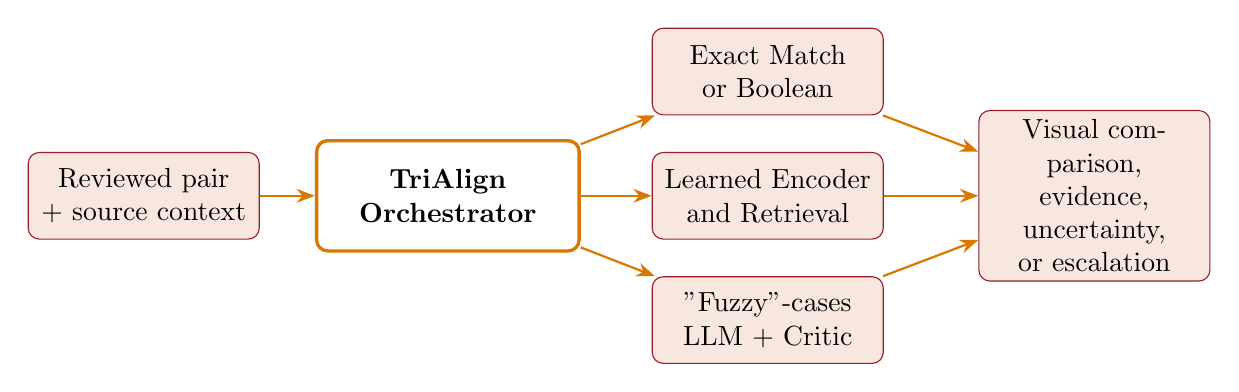
\begin{tikzpicture}[node distance=7mm,box/.style={draw=wine,rounded corners,fill=peach,text width=27mm,minimum height=11mm,align=center},agent/.style={draw=orange,very thick,rounded corners,fill=white,text width=31mm,minimum height=14mm,align=center,font=\bfseries},arr/.style={-{Stealth},thick,orange}]
\node[box] (i) {Reviewed pair\\+ source context};\node[agent,right=of i] (a) {TriAlign\\Orchestrator};
\node[box,above right=3mm and 9mm of a] (e) {Exact Match\\or Boolean};\node[box,right=9mm of a] (r) {Learned Encoder\\and Retrieval};\node[box,below right=3mm and 9mm of a] (l) {"Fuzzy"-cases\\LLM + Critic};\node[box,right=12mm of r] (o) {Visual comparison,\\evidence, uncertainty,\\or escalation};
\draw[arr](i)--(a);\draw[arr](a)--(e);\draw[arr](a)--(r);\draw[arr](a)--(l);\draw[arr](e)--(o);\draw[arr](r)--(o);\draw[arr](l)--(o);\end{tikzpicture}}\end{center}
The orchestrator decides which route fits the comparison: exact computation for fully structured cases, encoder retrieval for learned clinical similarity, or contextual LLM review for fuzzy language. It may combine routes to check conflicts, then returns an evidence-linked visual comparison or sends the case to a human. 
\end{frame}

\begin{frame}{The Human Feedback Loop}
\begin{center}\resizebox{.92\textwidth}{!}{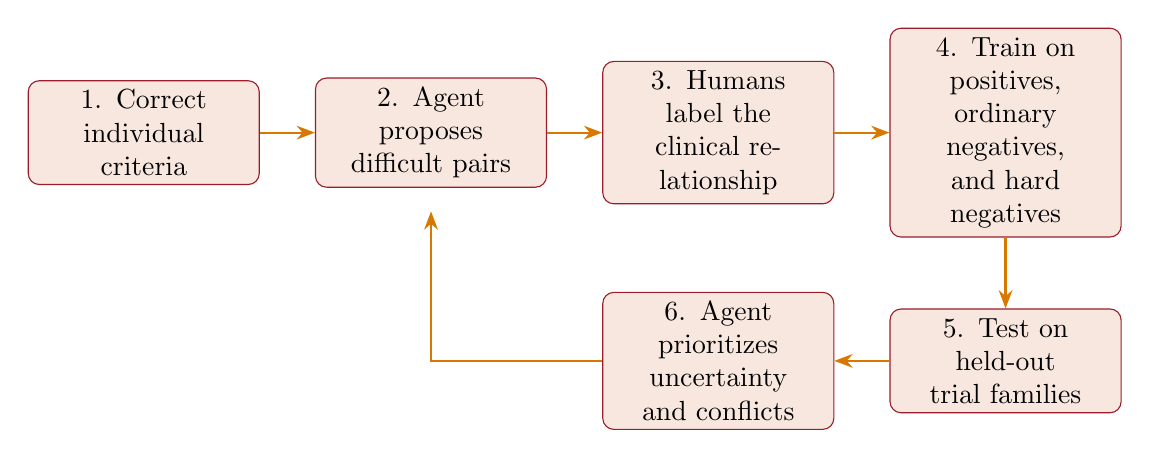
\begin{tikzpicture}[node distance=7mm,box/.style={draw=wine,rounded corners,fill=peach,text width=27mm,minimum height=12mm,align=center},arr/.style={-{Stealth},thick,orange}]
\node[box] (atoms) {1. Correct individual\\criteria};
\node[box,right=of atoms] (pairs) {2. Agent proposes\\difficult pairs};
\node[box,right=of pairs] (label) {3. Humans label the\\clinical relationship};
\node[box,right=of label] (train) {4. Train on positives,\\ordinary negatives,\\and hard negatives};
\draw[arr](atoms)--(pairs);\draw[arr](pairs)--(label);\draw[arr](label)--(train);
\node[box,below=9mm of train] (eval) {5. Test on held-out\\trial families};
\node[box,left=of eval] (mine) {6. Agent prioritizes\\uncertainty and conflicts};
\draw[arr](train)--(eval);\draw[arr](eval)--(mine);\draw[arr](mine.west)-|([yshift=-3mm]pairs.south);
\end{tikzpicture}}\end{center}
\begin{block}{Two different reviews}The current spreadsheet review validates each extracted criterion. The later pair review supplies labels such as equivalent, more restrictive, overlapping, disjoint, or ambiguous. Only accepted or adjudicated pair labels supervise the encoder.\end{block}
\source{Pilot and test pairs are independently double-labeled; unresolved cases remain ambiguous instead of being forced into a class.}
\end{frame}

\begin{frame}{Evaluation of TriAlign}
\begin{tabularx}{\textwidth}{@{}p{.30\textwidth}X@{}}\toprule Question & Test \\\midrule
How good are retrieved clinically comparable criteria? & Compare TF--IDF, frozen general/biomedical encoders, and our fine-tuned encoder using precision/recall@$k$, reciprocal rank, and anchor ordering. \\
Are important differences preserved? & Report errors by negation, thresholds, units, timing, repetition, exceptions, and logic; evaluate the separate relationship classifier with macro-F1 and order consistency. \\
Does the agent know when to escalate? & Measure calibration, risk--coverage, conflict detection, inappropriate acceptance, reviewer corrections, time, latency, and cost. \\
Did each component help? & Remove hard negatives, human corrections, critic checks, or targeted sampling and compare paired results across multiple seeds. \\\bottomrule\end{tabularx}
\vspace{.45em}\source{Trials are split by family before pairing; held-out labels are unavailable to agent retrieval. Natural and constructed cases are reported separately, with uncertainty preserving trial-family dependence.}
\end{frame}

\begin{frame}{Benchmark Comparisons}
\footnotesize
\begin{tabularx}{\textwidth}{@{}p{.20\textwidth}p{.27\textwidth}X@{}}\toprule System & Implementation & Comparison role \\\midrule
Lexical baseline & TF--IDF + cosine & Word-overlap reference. \\
General encoder & \texttt{all-mpnet-base-v2} & Frozen semantic-retrieval baseline. \\
Biomedical encoder & \texttt{BioLORD-2023} & Frozen biomedical-representation baseline. \\
TrialGPT-style agent & Criterion-level LLM reasoning adapted from patient--trial matching & Tests an LLM-only evidence-and-judgment workflow on compatible criterion-pair cases. \\
EligMeta-style agent & LLM parsing plus deterministic eligibility-alignment logic & Tests recent eligibility-aware agent design on compatible alignment cases. \\
TriAlign & Fine-tuned MPNet + directional head + routed tools & Learns reviewed hard cases and chooses deterministic, embedding, or fuzzy comparison. \\\bottomrule\end{tabularx}
\vspace{.4em}
\begin{block}{Fair comparison}All runnable systems receive the same reviewed pairs and evidence. We compare labels, ranking, evidence support, abstention, latency, and cost only where outputs align; TrialGPT and EligMeta remain task-adjacent rather than identical benchmarks.\end{block}
\source{Jin et al., TrialGPT, Nature Communications (2024); Zhao et al., EligMeta, arXiv:2604.02678 (2026); Hugging Face model cards for MPNet and BioLORD.}
\end{frame}

\begin{frame}{Five milestones from current review to delivery}
\small
\begin{tabularx}{\textwidth}{@{}p{.055\textwidth}p{.19\textwidth}p{.18\textwidth}X@{}}\toprule
& Stage & Timing & Exit artifact \\\midrule
\pill{1} & \textbf{Freeze inputs} & Oct. 20--Nov. 2 & Reviewed, blocker-free criterion corpus with versioned trial-family splits. \\
\pill{2} & \textbf{Build benchmark} & Nov. 3--9 & Adjudicated natural and challenge pairs plus frozen baseline results. \\
\pill{3} & \textbf{Improve distance} & Nov. 10--16 & Fine-tuned MPNet, directional relationship head, and validation-selected checkpoint. \\
\pill{4} & \textbf{Complete agent} & Nov. 17--30 & Routed exact/encoder/LLM tools, critic checks, calibration, abstention, and review workflow. \\
\pill{5} & \textbf{Validate + deliver} & Final period & Held-out tests, agent comparisons, ablations, intervals, UI, documentation, and demonstration. \\\bottomrule
\end{tabularx}
\vspace{.7em}
\begin{block}{Gate between stages}A stage advances only after its versioned artifacts and acceptance checks pass. Incomplete review or split leakage blocks training instead of being silently ignored.\end{block}
\end{frame}

\begin{frame}{A Quick UI “Sketch”}
\begin{columns}[T,onlytextwidth]\column{.31\textwidth}
\begin{block}{User request}
\textbf{Current trial:} NCT-new\\[.3em]
\textbf{Criterion:} Age $\geq18$ years\\[.3em]
\textbf{Ask:} Find comparable historical rules and explain the differences.
\end{block}
\begin{center}$\Downarrow$\\[-.2em]\small Agent routes tools and retrieves evidence\end{center}
\column{.65\textwidth}
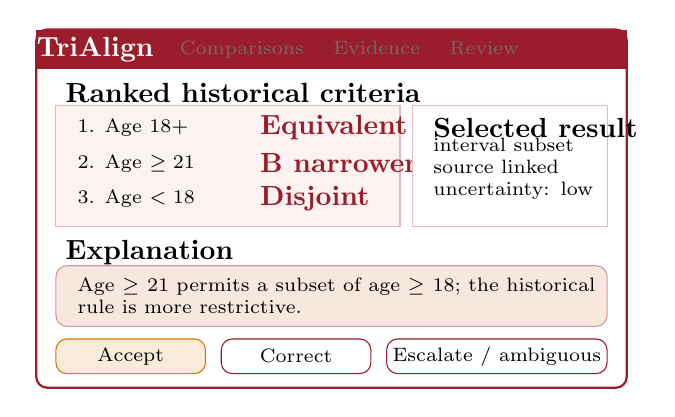
\begin{tikzpicture}[x=1cm,y=1cm,font=\scriptsize]
\draw[rounded corners,fill=white,draw=wine,thick] (0,0) rectangle (7.5,4.55);
\fill[wine] (0,4.05) rectangle (7.5,4.55);\node[text=white,font=\bfseries] at (.75,4.3) {TriAlign};
\node[anchor=west,text=muted] at (1.7,4.3) {Comparisons \quad Evidence \quad Review};
\node[anchor=west,font=\bfseries] at (.25,3.75) {Ranked historical criteria};
\draw[fill=peach!50,draw=wine!30] (.25,2.05) rectangle (4.62,3.58);
\node[anchor=west] at (.4,3.30) {1. Age 18+};\node[anchor=west,text=wine,font=\bfseries] at (2.72,3.30) {Equivalent};
\node[anchor=west] at (.4,2.85) {2. Age $\geq21$};\node[anchor=west,text=wine,font=\bfseries] at (2.72,2.85) {B narrower};
\node[anchor=west] at (.4,2.40) {3. Age $<18$};\node[anchor=west,text=wine,font=\bfseries] at (2.72,2.40) {Disjoint};
\draw[fill=white,draw=wine!30] (4.78,2.05) rectangle (7.25,3.58);
\node[anchor=west,font=\bfseries] at (4.92,3.30) {Selected result};
\node[anchor=west,text width=2.05cm] at (4.92,2.78) {interval subset\\source linked\\uncertainty: low};
\node[anchor=west,font=\bfseries] at (.25,1.72) {Explanation};
\draw[rounded corners,fill=peach,draw=wine!45] (.25,.78) rectangle (7.25,1.55);
\node[anchor=west,text width=6.7cm] at (.4,1.17) {Age $\geq21$ permits a subset of age $\geq18$; the historical rule is more restrictive.};
\draw[rounded corners,fill=orange!15,draw=orange] (.25,.18) rectangle (2.15,.62);\node at (1.2,.40) {Accept};
\draw[rounded corners,fill=white,draw=wine] (2.35,.18) rectangle (4.25,.62);\node at (3.30,.40) {Correct};
\draw[rounded corners,fill=white,draw=wine] (4.45,.18) rectangle (7.25,.62);\node at (5.85,.40) {Escalate / ambiguous};
\end{tikzpicture}
\end{columns}
\vspace{.25em}\source{The dashboard separates retrieval score from clinical relationship, exposes source evidence and agent checks, and preserves every human correction in the audit trail.}
\end{frame}
\end{document}
